\begin{theorem} \leavevmode \\
    \label{thm2.19}
    Let $(X,d)$ be a metric space. Let $p \in X$ and $\epsilon > 0$. Then $\nbhd{\epsilon}{p}$ is an open set.
\end{theorem}

\begin{proof}
    Our goal is to show that every point of $N_\epsilon (p)$ is an interior point of $N_\epsilon (p)$.
    Let $q\in N_\epsilon (p)$. We need to show that $$\exists \delta > 0 \text { such that } N_\delta(q) \subseteq N_\epsilon(p)$$
    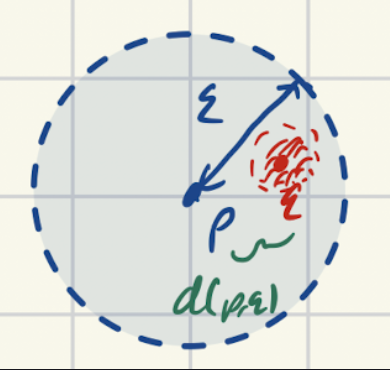
\includegraphics[width=.30\linewidth, center]{/Users/josiahvillarante/GradSchool/Grad-School-Notes/Math230A/Lecture/CH2/images/open set.png}
    Let $\delta = \epsilon - d(p,q)$. We claim that $N_\delta (q) \subseteq N_\epsilon (p)$.
    Indeed, if $x\in N_\delta (q)$ then
    \begin{align*}d(q,x) < \delta &\implies d(q,x) < \epsilon - d(p,q) \\ &\implies d(p,q) + d(q,x) < \epsilon \\ &\implies d(p,x)< \epsilon \\ &\implies x\in N_\epsilon(p). \end{align*}
    \qed
\end{proof}

\begin{description}
    \item[HW 4: $(18-b)$] \leavevmode \\
    If $G\subseteq E$ and $G$ is open, then $G \subseteq \overset{\circ}{E}$.
\end{description}

\begin{theorem} \leavevmode \\
    \label{thm2.20}
    Let $(X,d)$ be a metric space and let $E \subseteq X.$ If $p \in E'$, then every neighborhood of $p$ contains infinitely many points of $E$.
\end{theorem}

\begin{proof}
    Assume for contradiction that 
    $$\exists \epsilon > 0 \st \nbhd{\epsilon}{p} \cap E \text{ is a finite set.}$$
    Since $\nbhd{\epsilon}{p}\cap \left(E \backslash \{p\}\right) \subseteq \nbhd{\epsilon}{p} \cap E$, we can conclude that $\nbhd{\epsilon}{p}\cap \left(E \backslash \{p\}\right)$ is finite also. Let's denote the elements of $\nbhd{\epsilon}{p}\cap \left(E \backslash \{p\}\right)$ by $x_1, ..., x_n$. For each $i \in \{1,..., n\}, ~d(p, x_i) > 0,$ so $\delta = \min \{d(p, x_1), ..., d(p, x_n)\} > 0.$ Clearly, $\nbhd{\epsilon / 2}{p} \cap \left(E \backslash \{p\}\right) = \emptyset.$ This contradicts the assumption that $p \in E'$.
    \qed
\end{proof}

\begin{corollary} \leavevmode \\
    A finite set has no limit points.
    \begin{enumerate} [$*)$]
        \item If $E$ is finite, then $E' = \emptyset$
        \item If $E$ is infinite, then $E' \subseteq E$ so $E$ is closed
    \end{enumerate}
\end{corollary}

\begin{theorem} \leavevmode \\
    \label{thm2.23}
    \routineMS and let $E\subseteq X.$ $E$ is open if and only if $E^c$ is closed.
\end{theorem}

\begin{proof}
    $(\implies)$ Suppose $E$ is open. Our goal is to show that $(E^c)' \subseteq E^c.$ Let $p \in (E^c)'$. Our goal is to show that $p \in E^c$. Assume for contradiction $p \not \in E^c.$ Then $p \in E.$ Since $E$ is open, $p$ is an interior point of $E$:
    \begin{align*}
        &\exists \delta > 0 \st \nbhd{\epsilon}{p} \subseteq E \\ 
        &\implies \exists \delta > 0 \st \nbhd{\delta}{p}\cap E^c = \emptyset \\
        &\implies \exists \delta > 0 \st \nbhd{\delta}{p} \cap \left(E^c \backslash \{p\}\right) = \emptyset \\
        &\implies p \not \in (E^c)',
    \end{align*}
    which contradicts the assumption that $p \in (E^c)'$. \\
    $(\impliedby)$ Suppose $E^c$ is closed. Our goal is to show that every point of $E$ is an interior point. Let $p \in E.$ Assume for contradiction that $p$ is not an interior point of $E$. Then
    $$\forall \epsilon > 0 ~~\nbhd{\epsilon}{p} \not \subseteq E.$$
    Hence,
    \begin{align*}
        &\forall \epsilon > 0 ~\nbhd{\epsilon}{p} \cap E^c \not = \emptyset \\
        \implies &\forall \epsilon > 0 ~\nbhd{\epsilon}{p}\cap \left(E^c \backslash \{p\}\right) \not = \emptyset &&(p\in E) \\
        \implies &p \in \left(E^c\right)' \\
        \implies &p\in E^c &&(E^c \text{ is closed})
    \end{align*}
    This contradicts the assumption that $p\in E$.
    \qed
\end{proof}

\begin{theorem} \leavevmode \\
    \label{thm2.24}
    Let $(X,d)$ be a metric space
    \begin{enumerate}[$(i)$]
        \item Suppose $\ocover{A}$ is a collection of open sets. Then $\bigcup \limits_{\alpha \in \Lambda}A_{\alpha}$ is an open set.
        \item Suppose $A_1, ..., A_n$ are open sets. Then $\bigcap \limits_{k=1}^n A_k$ is open.
    \end{enumerate}
\end{theorem}

\begin{proof}
    \begin{enumerate}[$(i)$]
        \item Our goal is to show that every point of $\bigcup \limits_{\alpha \in \Lambda} A_{\alpha}$ is an interior point. Let $p\in \bigcup \limits_{\alpha \in \Lambda}A_{\alpha}$. We have:
        \begin{align*}
            p\in \bigcup \limits_{\alpha \in \Lambda}A_{\alpha} &\implies \exists \alpha_0 \in \Lambda \st p \in A_{\alpha_0} \\
            &\implies \exists \delta > 0 \st \nbhd{\delta}{p} \subseteq A_{\alpha_0} &&(A_{\alpha_0} \text{ is open}) \\
            &\implies \nbhd{\delta}{p} \subseteq \bigcup \limits_{\alpha \in \Lambda}A_{\alpha} &&\left(A_{\alpha_0} \subseteq \bigcup \limits_{\alpha \in \Lambda}A_{\alpha}\right) \\
            &\implies p \text{ is an interior point of } \bigcup \limits_{\alpha \in \Lambda}A_{\alpha}
        \end{align*}
        
        \item Our goal is to show that every point of $\bigcap \limits_{k=1}^n A_k$ is an interior point of $\bigcap \limits_{k=1}^n A_k$. Let $p \in \bigcap \limits_{k=1}^n A_k.$ We have
        \begin{align*}
            p \in \bigcap \limits_{k=1}^n &\implies \forall k \in \{1,...,n\} ~~p \in A_k \\
            &\implies \forall k \in \{1,...,n\} ~~\exists \delta_k > 0 \st \nbhd{\delta_k}{p} \subseteq A_k.
        \end{align*}
        Let $\delta = \min \{\delta_1, ..., \delta_k\}.$ We have
        $$\forall k \in \{1,...,n\} ~~\nbhd{\delta}{p} \subseteq \nbhd{\delta_k}{p}\supseteq A_k.$$
        Consequently,
        $$\nbhd{\delta}{p} \subseteq \bigcap \limits_{k=1}^n A_k.$$
        Hence, $p$ is an interior point of $\bigcap \limits_{k=1}^n A_k$.
        \qed
    \end{enumerate}
\end{proof}

\begin{theorem}
    \routineMS and let $E\subseteq X.$
    \begin{enumerate}[$(i)$]
        \item $\overline{E}$ is a closed set $(\overline{E}=E \cup E')$
        \item $E$ is closed if and only if $E=\overline{E}$
        \item If $E\subseteq F$ and $F$ is closed, then $\overline{E} \subseteq F$.
    \end{enumerate}
    \begin{note}
        $(i)$ and $(iii)$ tell us $\overline{E}$ is the smallest closed set that contains $E$.
    \end{note}
\end{theorem}

\begin{proof}
    \begin{enumerate}[$(i)$]
        \item Our goal is to show that $\left(\overline{E}\right)^c$ is open. We need to show that every point of $\left(\overline{E}\right)^c$ is an interior point of $\left(\overline{E}\right)^c$. Let $p\in \left(\overline{E}\right)^c.$ We have 
        \begin{align*}
            p\in \left(\overline{E}\right)^c &\implies p \not \in \overline{E} \\
            &\implies p \not \in (E\cup E') \\
            &\implies p \not \in E \wedge p \not \in E'.
        \end{align*}
        Note That
        \begin{align*}
            p\not \in E' &\implies \exists \epsilon > 0 ~~\nbhd{\epsilon}{p}\cap \left(E \backslash \{p\}\right) = \emptyset \\
            &\implies \exists \epsilon > 0 ~~\nbhd{\epsilon}{p} \cap E = \emptyset. \tag{$I$}
        \end{align*}
        In what follows we will show that $\nbhd{\epsilon}{p}\cap E'= \emptyset$ also, so 
        \begin{align*}
            &\nbhd{\epsilon}{p}\cap \left(E \cup E'\right) = \emptyset \\
            \implies &\nbhd{\epsilon}{p}\cap \overline{E} = \emptyset \\
            \implies &\nbhd{\epsilon}{p} \subseteq \left(E\right)^c \\
            \implies &p \text{ is an interior point of } \left(E\right)^c.
        \end{align*}
        It remains to show that $\nbhd{\epsilon}{p}\cap E' = \emptyset.$ Assume for contradiction that $\nbhd{\epsilon}{p} \cap E' \not = \emptyset.$ Let $q \in \nbhd{\epsilon}{p} \cap E'.$ We have
        \begin{align*}
            q\in \nbhd{\epsilon}{p} &\implies \exists \delta > 0 \st \nbhd{\delta}{q} \subseteq \nbhd{\epsilon}{p} \\
            q \in E' &\implies \nbhd{\delta}{q}\cap \left(E \backslash \{q\}\right) \not = \emptyset \tag{$*$}
        \end{align*}
        Notice that since $\nbhd{\delta}{q} \subseteq \nbhd{\epsilon}{p}$ and $E \backslash \{q\} \subseteq E$, $(*)$ implies that 
        $$\nbhd{\epsilon}{p}\cap E \not = \emptyset.$$
        This contradicts $(I)$.

        \item $E$ is closed $\iff E' \subseteq E \iff E' \cup E = E \iff \overline{E} = E.$

        \item Suppose $E\subseteq F,$ and $F$ is closed. We want to show $\overline{E} \subseteq F$. Let $p \in \overline{E}$. Our goal is to show that $p \in F.$ We have
        $$p\in \overline{E} \implies p \in E \vee p \in E'.$$
        \begin{enumerate}[$*$]
            \item If $p\in E,$ then $p\in F$
            \item If $p\in E',$ then 
            \begin{align*}
                &\forall \epsilon > 0 ~~\nbhd{\epsilon}{p}\cap \left(E \backslash \{p\}\right) \not = \emptyset \\
                \implies &\forall \epsilon > 0 ~~\nbhd{\epsilon}{p} \cap \left(F \backslash \{p\}\right) \not = \emptyset &&(E \backslash \{p\} \subseteq F \backslash \{p\}) \\
                \implies &p\in F' \\
                \implies &p \in F &&(F \text{ is closed}).
            \end{align*}
        \end{enumerate}
    \end{enumerate}
    \qed
\end{proof}